\section{Versuchsaufbau/-durchführung}

\subsection{Versuchsaufbau}
Der grundlegende Aufbau ist in der Abbildung \ref{fig: aufbau} abgebildet.
\begin{figure}[!h]
  \centering
  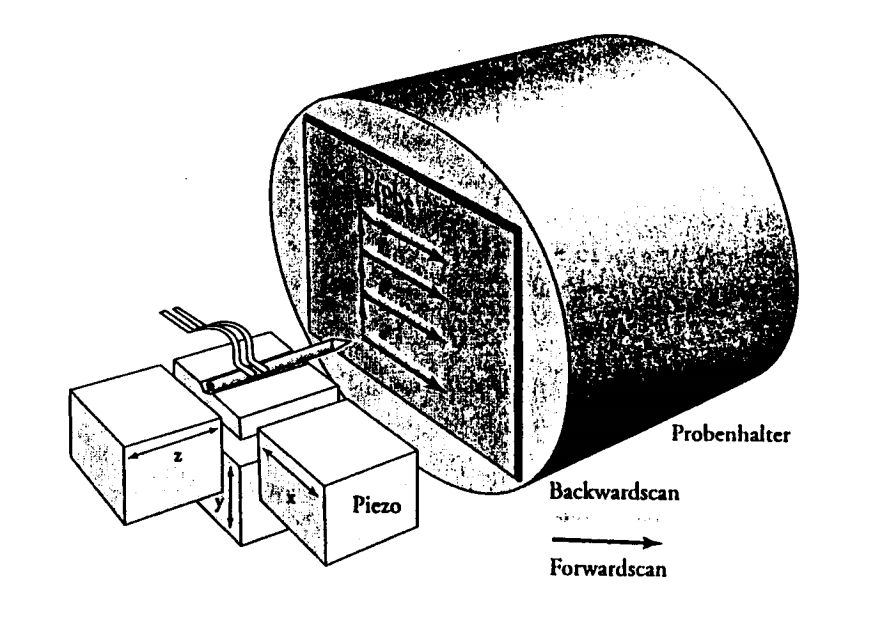
\includegraphics[width=0.6\textwidth]{./pics/aufbau.png}
  \caption{Grundlegender Aufbau eines Rastertunnelmikroskops \cite{anleitung_frankfurt}.}
  \label{fig: aufbau}
\end{figure}
In der Abbildung ist die Spitzenhalterung zu sehen und
der Carrier mit Probe. Die Apperatur wird mittels Computersoftware gesteuert.
Die Spitze wird mit Hilfe von Piezokeramiken filigran bewegt, somit
ist ein präzises Abrastern der Probe möglich.

Beim Abfahren der Probe, gibt es zwei Methoden die Struktur der Probe zu erfassen.
Zum einen ist es möglich den Abstand zwischen Probe und Spitze konstant zu lassen
und die Veränderung des Tunnelstroms zu messen.
Jedoch bietet diese Methode die Gefahr, dass die Spitze die Probe rammt und so unbrauchbar wird
Umgekehrt ist es möglich den Tunnelstrom konstant zu lassen und den Abstand zu variieren.
Die in der Theorie angesprochende Näherung, dass die Auslenkung des Piezokrostalls linear
mit dem anliegenden Feld geht ist in der Realität kaum zu beobachten. Deshalb wird eine
geeignete Regelkreis benötig, die eine genaue Ansteuerung des Piezokristall ermöglicht.
Der verwendete Regelkreis misst die den Tunnelstrom $I$ und vergleicht diesen mit einen
eingestellten Sollwert. Bei einer Differenz der beiden Werte wird die Höhe des Piezoelemnts
entsprechend angepasst. Dabei lässt sich die Anpasssgeschwindigkeit über zwei Parameter
einstellen. Zum einen den \emph{integralen Anteil}, dieser beeinflusst im wesentlich die
Geschwindigkeit mit der auf Abweichung reagiert wird. Zum andern kann mit Hilfe
dem \emph{propotionalen Anteil} gibt an wie stark auf eine Abweichung reagiert wird.
Die Werte vom integralen und propotionalen Anteil hängen von der Beschaffenheit
der Probe und Spitze ab \cite{anleitung_frankfurt}.

\subsection{Versuchsdurchführung}

Für eine genaue Messung wird eine einatomige Spitze benötigt.
Die Spitze wird aus \ce{PtIr}-Draht (Platinum-Iridium) hergestellt, dazu
werden eine Pinzette, eine Zang und ein Seitenscheider verwendet.
Bevor diese benutzt werden können müssen sowohl sie als auch der Draht mit Aceton und Propanol
gereinigt werden. Damit die Spitze besonder fein wird, werden die Werkzeuge wie in Abbildung \ref{fig: zange_schneider}
dargestellt positioniert.
\begin{figure}[!h]
  \centering
  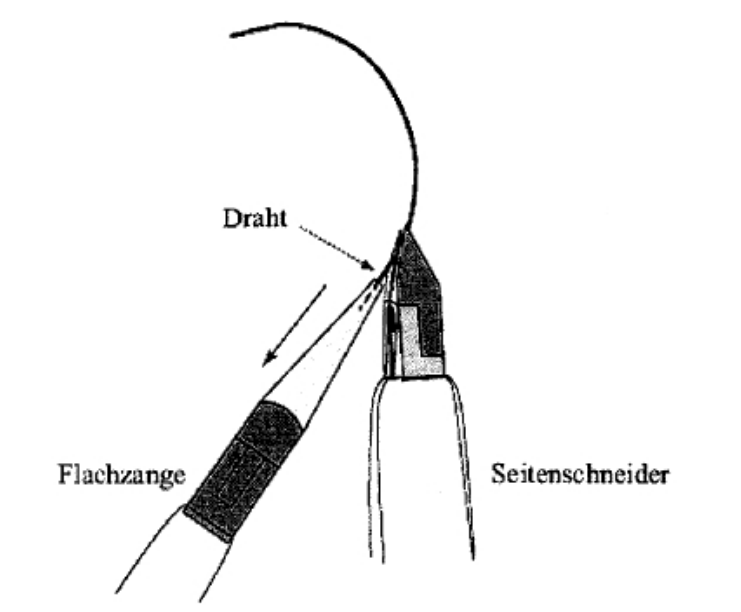
\includegraphics[width=0.6\textwidth]{./pics/herstellung_spitze.png}
  \caption{Positionierung des Seitenschneiders und der Zange am Draht. \cite{anleitung_frankfurt}.}
  \label{fig: zange_schneider}
\end{figure}
Anschließend werden Zange und Schneider in entgegensetzte Richtung gezogen, der Draht sollte
auseinander gerissen werden. Wichtig ist das der Draht nicht geschnitten wird.

Nachdem eine Spitze gerissen wurde wird diese in das Rastertunnelmikroskop eingesetzt.
Anschließend wird der Carry mit der Probe in das RTM eingeführt.
Nun muss die Probe nah genug an die Spitze herangeführt werden, dies wird zu Beginn
manauell gemacht. Die Probe wird manauell so nah an die Spitze herangeführt, bis sich
die Spitze und ihr Spiegelbild beinah berühren. Die Software für das automatische
heranführen, überprüft regelmäßig ob ein Tunnelstrom detektiert werden kann oder nicht.
Wird zum Beispiel kein Tunnelstrom gemessen, so wird die Probe, von der Software
näher an die Spitze gefahren ($I\propto d$). Deshalb ist es wichtig bevor der automatische
Modus verwendet wird, eine Spannung an der Spitze anzulegen. Mit Hilfe einer
Statusleuchte kann kontrolliert werden, ob eine Tunnelstrom detektiert wurde und
ob die Spitze die Probe berührt hat.
Sobald die Software fertig mit der Justage ist, beginnt die Messung automatisch.
Bei der Messung wird unterschieden, ob die Spitze von rechts nach links oder von links nach rechts
die Probe abrastert (vgl. Abb. \ref{fig: aufbau}). Die Unterscheidung wird auf Grund der thermischen Dirfts vollzogen.
Sobald die rechts nach links bzw. links nach rechts Messung/Bilder identisch sind,
unterliegt die Probe keiner thermischen Ausdehnung. Auf jeder, der in der Skizze \ref{fig: aufbau} zu sehende, Linie misst die Spitze eine
vorher eingestellte Anzahl mal den Abstand zwischen Probe und Spitze, hierzu wird die Methode des konstanten
Tunnelstroms verwendet.

In dem Versuch werden eine HOPG- und eine Gold- Probe vermessen.
Bei der HOPG-Probe sollen die Gittervektoren der atomaren Struktur
experimentell bestimmt werden. Die Bestimmung der Gittervektoren
bei Gold nicht mit dem verwendeten Versuchsaufbau möglich, statdessen
wird das Höhenprofil der Goldoberfläche gemessen.
